\documentclass{report}
\usepackage[margin=1in, paperwidth=8.5in, paperheight=11in]{geometry}
%Math packages%
\usepackage{amsmath}
\usepackage{amsthm}
%Spacing%
\usepackage{setspace}
\onehalfspacing
%Lecture number%
\newcommand{\lectureNum}{7}
%Variables - Date and Course%
\newcommand{\curDate}{January 24, 2017}
\newcommand{\course}{CS 251}
\newcommand{\instructor}{Stephen Mann}
%Defining the example tag%
%\theoremstyle{definition}%
\newtheorem{ex}{Example}[section]
%Setting counter given the lecture number%
\setcounter{chapter}{\lectureNum{}}
%Package to insert code%
\usepackage{listings}
\usepackage{courier}
\usepackage{xcolor}
\lstset { %
    tabsize=2,
    breaklines=true,
    language=C++,
    backgroundcolor=\color{blue!8}, % set backgroundcolor
    basicstyle=\footnotesize\ttfamily,% basic font setting
}
%Package used to draw circuits%
\usepackage{circuitikz}
\begin{document}
%Note title%
\begin{center}
\begin{Large}
\textsc{\course{} | Lecture \lectureNum{}}
\end{Large}
\end{center} 
\noindent \textit{Bartosz Antczak} \hfill
\textit{Instructor: \instructor{}} \hfill
\textit{\curDate{}}
\rule{\textwidth}{0.4pt}
% Actual Notes%
\subsubsection{Note: unused states}
In the graphical representation for a finite state machine, for any states that aren't included, they are \textit{unused states}.
\section{Number Representation}
Focusing on binary numbers, we can define what each 32-bit binary string represents.
\subsubsection{Unsigned Binary Numbers}
\textit{Unsigned} means a positive number. Binary numbers are stored in 32-bits of memory, thus we can represent the numbers 0 through $2^{32}-1 = 4,294,967,295$.
\subsubsection{Signed Binary Numbers}
\textit{Signed} numbers include negative numbers. How do we represent binary numbers as a negative? We use \textbf{two's compliment} (outlined more in detail in the lecture 1 notes for CS 241, subsection 1.2.1).\\
The idea is that we let MSB represent the negative of a power of 2. For instance, with 4 bits, bit 3 (MSB) represents $2^{-3}$, which is 1110 in two's compliment. With 32 bits, we can represent the numbers $-2,147,483,648$ to $2,147,483,647$. When we add 32-bit binary numbers and result in a sum that is larger than 32 bits, the processor simply cuts off the leading digits until we have 32 bits.\\
To visualize this, let's simplify to 4-bit binary numbers: if we calculate $1111 + 1 = 10000$, we cut off the leading 1, thus our answer is $0000$. This is called \textit{overflow}. This overflow creates a pseudo-modulo counting system:
\begin{figure}[ht]
\begin{center}
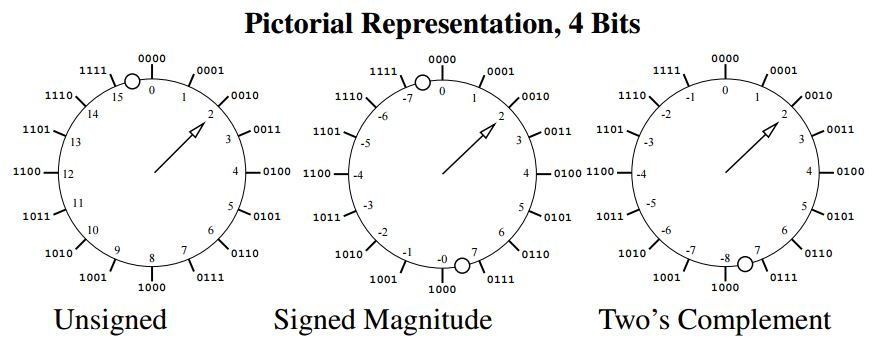
\includegraphics[scale=0.5]{4-bit-representation.jpg}
\end{center}
\caption{Source: The 4-bit binary representation for each number. Courtesy of Prof. Mann's slides.}
\end{figure}
Signed binary digits are negative if the first bit is a 1; positive otherwise.
\subsection{Sign Extension}
With 4 bits, 0110 is $+6$, but what is it with 8 bits? Similarly with 4 bits, 1010 is $-6$, and again we ask, what is it with 8 bits? \\
For $+6$, it's simple: just add the correct number of zeros to the front of the binary string (i.e., $+6$ in 8 bits becomes 0000 0110).\\
Similarly for $-6$, rather than zeros, add the correct number of ones to the front of the binary string (i.e., $-6$ in 8 bits becomes 1111 1010).
\subsection{Adding Binary Numbers}
Adding binary numbers, we simply use the ``elementary school algorithm" (outlined in my notes for CS 241 lecture 1, in example 1.2.2). To subtract numbers, we negate and then add.\\
As previously mentioned, overflow may occur because the sum of both addends contains more bits (i.e., adding two 32-bit strings can yield a 33-bit string, which is overflow!).\\
 Overflow cannot occur, so the leading extra bits are cut off. This means that overflow occurs when both of the addends have the same sign but the answer has a different sign.
\subsection{Building an Addition Circuit}
Let's build a simple adder that takes three bits as input and outputs a 2-bit sum (i.e., add A, B, and Cin, and output in two bits as Cout, S).
The truth table defining the circuit is
\begin{center}
\begin{tabular}{ c c c | c c }
A & B & Cin & Cout & S \\ \hline
0 & 0 & 0 & 0 & 0 \\
0 & 0 & 1 & 0 & 1 \\
0 & 1 & 0 & 0 & 1 \\
0 & 1 & 1 & 1 & 0 \\ \hline
1 & 0 & 0 & 0 & 1 \\
1 & 0 & 1 & 1 & 0 \\
1 & 1 & 0 & 1 & 0 \\
1 & 1 & 1 & 1 & 1 \\
\end{tabular}
\end{center}
The Boolean formulas for the outputs are defined as:
\begin{center}
Cout $=$ AB $+$ ACin $+$ BCin (this means that Cout is only 1 if at least 2 digits are 1) \\
S = A$\oplus$B$\oplus$in (if there are one or three 1's)
\end{center}
The circuit constructed from these formulas is shown on the next page.
\begin{figure}[ht]
\begin{center}
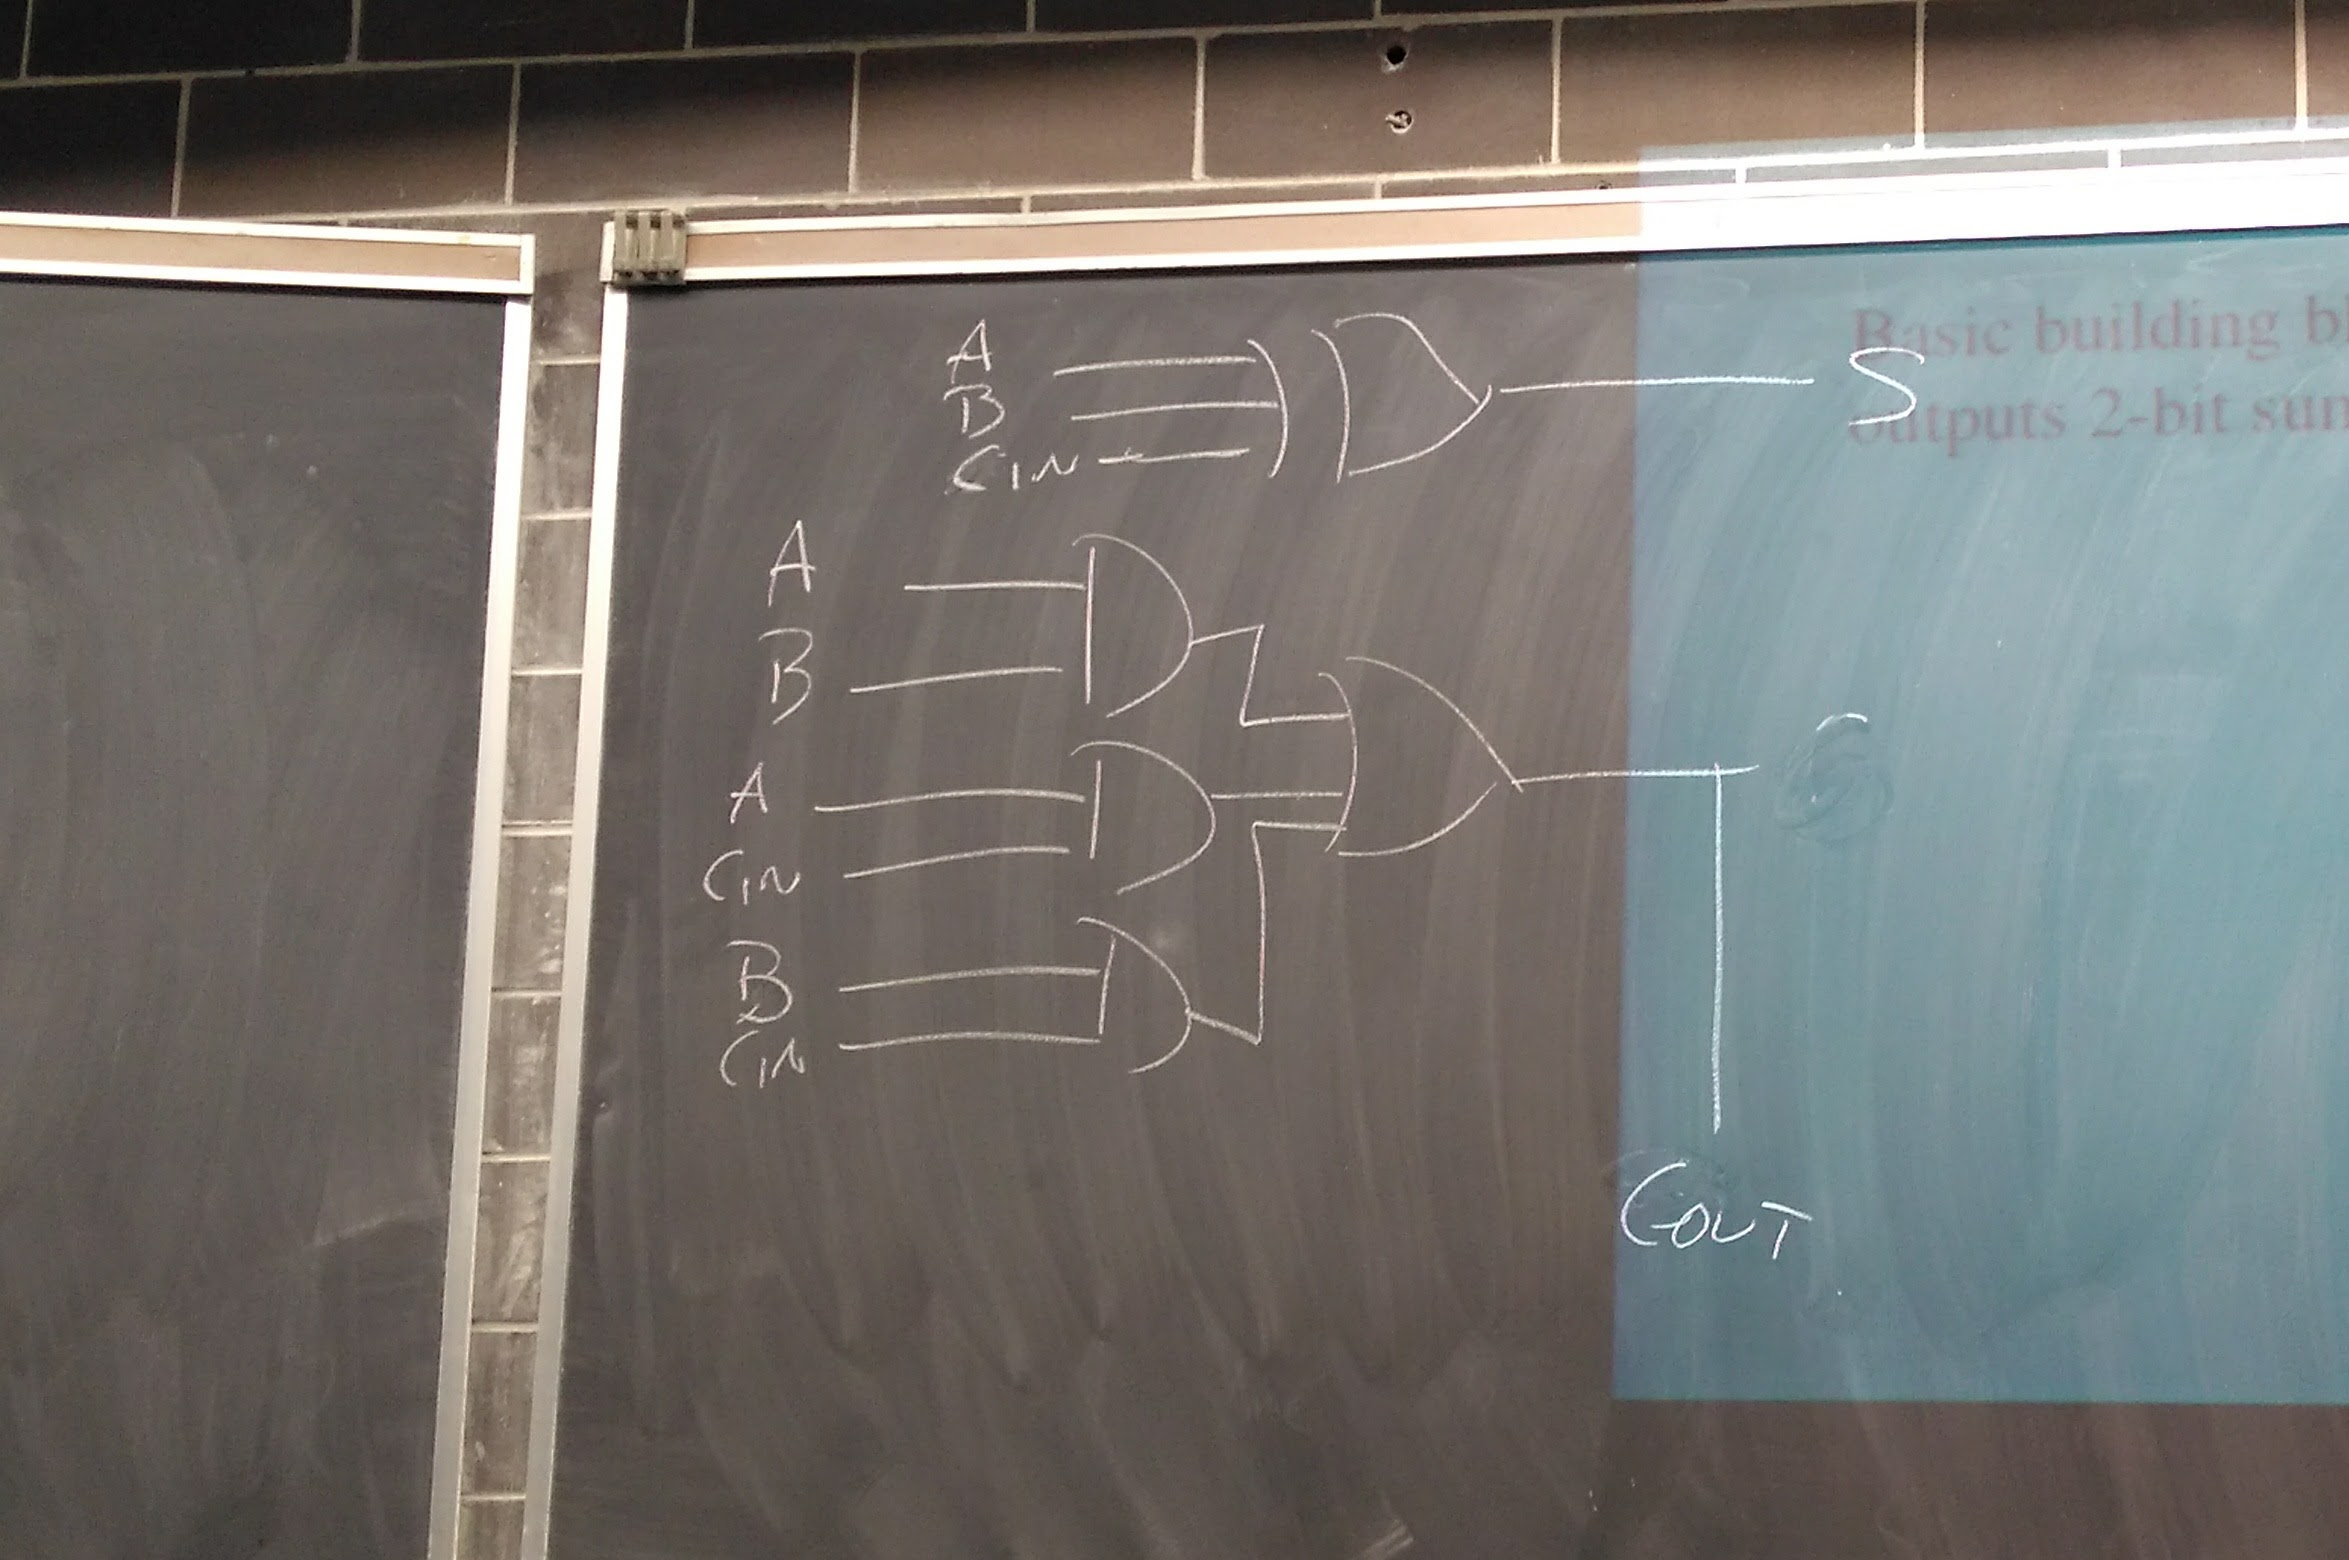
\includegraphics[scale=0.13]{circuit.jpg}
\end{center}
\caption{Courtesy of Prof. Mann's slides.}
\end{figure}\newpage
\subsection{Logical Operations}
This subsection outlines \textit{bitwise and}, \textit{bitwise or}, and \textit{shifting} operations on binary numbers. My CS 241 notes from lecture 6, subsection 6.2.1 outline the exact same thing we're learning in this in this topic.
%END%
\end{document}